\section{Key Concepts}

The topologygenerator is a tool for building a custom output file format out of a given network topology. The key concepts in this tool are the followings:
\begin{itemize}
\item Provider \\
Will be in charge of everything which is concerned to the network topology, meanning that it will have to provide information about it's elements, how they are connected between each other, general properties of each of the elements, etc., as well as has the ability to change it's content, for example adding new elements to the network, creating new connections, deleting elements, etc.
\item NetworkTopology \\
Is an abastract representation of the network which will be build by several requests to the provider.
\item Builder \\
Builders will know how to create from a network topology the desired output. For each type of element in the network (for example host, link, device), we will have a builder.\\
This element is easily implemented thanks to the network topology explained above, since this abstraction allow us to decouple from the real provider (it wouldn't be the same to build an element if the provider is Onos or OpenDayLight, since the way of getting the information from the element varies depending on the controller). \\
\item Output \\
Is what we are seeking, our main objective. This output can be either a file or multiple files, and will be generated by either one or multiple builders.
\end{itemize}

\subsection{Examples of use}

Understood the key concepts, let's understand how this elements relates one with each other with some examples of use. We will first start focusing in an abstract example, where we just have one provider and N type's of elements in the network as showed in the next image:

\begin{figure}[H]
\centering
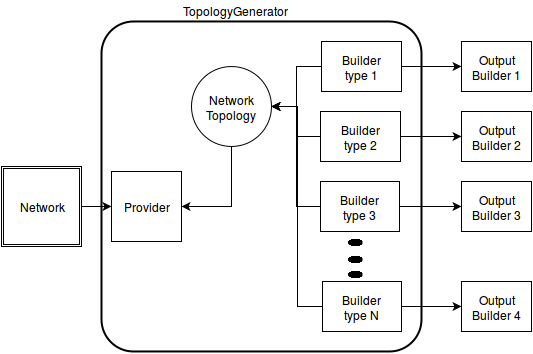
\includegraphics[width=\textwidth]{images/topologygenerator/topologygenerator_abstract_multiple.png}
\caption{Abstract interaction of elements with multiple outputs}
\end{figure}

In this image we can see how the elements explanied above interact. The provider will communicate with the real network, in the image above the real network is represented as the network which is outside the topology generator, to get all the information necessary in order to create the network topology representation. This comunication can either happen locally or remotely as we will see in one of the followings examples.\\
Once the representation is created, the builders are called to generate the output. In this example, we consider having N different types of elements in the network topology, which make us to have N different types of builders (1 per each type). Just to remark what was explained about the output, we are showing an example where we have one output per builder. This is not necessary the only case, as we can see in this other example: 

\begin{figure}[H]
\centering
\includegraphics[width=\textwidth]{images/topologygenerator/topologygenerator_abstract_single.png}
\caption{Abstract interaction of elements with single output}
\end{figure}

As we can see in this case, the logic of joining all the outputs from each of the builder's type is made by a new builder called TopologyBuilder, which is the one who finally generate's the desired output.\\

Let's consider now a concrete example where we want to obtain a network from either ONOS or OpenDayLight controller, and then create a DEVS's model for running simulations. We will assume that we are interested in hosts, devices and links of the network, meaning that we will consider only three types of elements. \\
In this example, we will need to have two providers, one per each controller, three builders, one per each type, and one more builder which will have the logic of joining all the output's provided to generate one common output, the topology.pdm, as show next:

\begin{figure}[H]
\centering
\includegraphics[width=\textwidth]{images/topologygenerator/controller_example.png}
\caption{Controller's example}
\end{figure}

Each of the providers in the image above, will have the knowledge to communicate with it's corresponding controller. In this example, the OnosProvider will encapsulate the logic to communicate with the Api Rest from the Onos controller, meanwhile the OpenDayLightProvider will do the same for the OpenDayLight controller.\\
The interaction with the controller can be either locally, for example this can happens if the controller is set up in the same machine where the topologygenerator is running, or remotely, for example if the controller is set up in a different machine and the comunication is made via http. How to implement both possibilities will be further explained in the next section.\\
The output generated is a pdm which can be interpretated by the DEVS simulator.\\

What happen if we do not have a real network?, What if we have a representation of a network in a programming language, for example Ruby, and we want to create from this network a simulation to test properties?. Then we can use the topologygenerator as follow in the next image:

\begin{figure}[H]
\centering
\includegraphics[width=\textwidth]{images/topologygenerator/ruby_provider.png}
\caption{Ruby as provider and DEVS as output}
\end{figure}
 
This image shows how it's just a question of creating a new provider, in this case the ruby provider, which will be in charge of having the knowledge of how to make the request to the script to obtain all the necessary information in order to create the network topology representation. Since we still want to create a simulation, the builders and the output is still the same. \\

In this previous example we show a powerful characteristic of the tool, which is that providers and builders are not related at all, meaning that changing a provider does not imply to change builders. This characteristic allow us then to create as much providers and builders as we want, and to connect them independently each other to generate as many desired output as we may want. \\

What would happend if we want to try out our custom topology written in Ruby, and test it in an Onos enviorment?, How could we manage to do this?.\\
In this example we would like to have our ruby provider, as in the previous case, and builders that generates request to the ONOS Api as show in the following image:

\begin{figure}[H]
\centering
\includegraphics[width=\textwidth]{images/topologygenerator/onos_builder.png}
\caption{Ruby as provider and ONOS as output}
\end{figure}

Each of the builder's in this case will generate requests to the ONOS Api that will create each of the elements in the SDN enviorment (this is a good example of the capability of SDN, since the enviorment allow us to create elements in the network). \\
In this example, it's important to notice how malleable and easy results to change ONOS, which was though as a provider in previous examples, to a desired output.\\

With the examples showed, we have a good understanding in the power of the tool and how it is supposed to be used. In the following section we will provide a tutorial for using the topologygenerator, and we will implement some of the examples showed before.

\section{Tutorial}

In this tutorial we will demonstrate how to install and use the topologygenerator tool. The tutorial was tested in a machine running Ubuntu 16.04, however should work in any machine which has a ruby version of 2.0 or major installed. \\

\subsection{Installation}

You will need to have Ruby installed in your machine. We recommend for this installing the ruby version manager (RVM), however any installation should be fine.\\

Once ruby is installed, you can proceed now to install the topologygenerator. For doing this, you will have two options: 
\begin{itemize}
\item Installing it as a gem \\
You should go for this option in case you are thinking in using the topologygenerator as a library of your Ruby project. 
\item Installing it as a binary \\
Select this option in case you are not interested in adding the topologygenerator as a library of any project. In this case, you will use the topologygenerator as a binary.
\end{itemize}

Per each option please refer to the corresponding subsection listed below.

\subsubsection{Installation as a gem}

Add this line to your application's Gemfile:

\begin{lstlisting}[language=Ruby,breaklines=true]
gem 'topologygenerator'
\end{lstlisting}

And then execute:

\begin{lstlisting}[language=bash,breaklines=true]
$ bundle
\end{lstlisting}

Or install it yourself as: 

\begin{lstlisting}[language=bash,breaklines=true]
$ gem install topologygenerator
\end{lstlisting}

\subsubsection{Installation as a binary}

\textbf{Pre-requisite}: Have installed and configured a git client. \\

Execute the followings lines (replace \textbf{TOPOLOGY\_DIRECTORY} with the corresponding path):

\begin{lstlisting}[language=bash,breaklines=true]
$ git clone git@github.com:andyLaurito92/topologygenerator.git
$ sudo ln -s "$TOPOLOGY_DIRECTORY/lib/createTopology.rb" /usr/bin/topologygenerator
\end{lstlisting}

\subsection{Using the tool}

How to use the topologygenerator will depend in which of the installation's guide you have done, however both ways are not so different and remember that you can always have the tool installed as a gem and a binary at the same time. In case you have installed the tool as a binary, we encourage you to first read the Use as a gem section, and then proceed to the Use as a binary section, since it still will be useful. \\
Both tutorials require you to have installed either Onos or OpenDayLight Controller and mininet. \\
First we will guide you in how to use the tool using the builders and providers implemented as examples, and then you will get hands on into the code and implement a provider and a builder. In both using examples, we will use the ONOS and OpenDayLight providers, and the PDM and Ruby builders. \\

NO ESTOY SEGURO SI SE PUEDEN USAR LOS BUILDERS Y PROVIDERS POR DEFECTO EN LA INSTALACIÓN DE LA GEMA, PORQUE NO SE SI RUBY TE DEJA ACCEDER A TODO EL PROYECTO DE LA GEMA, O SOLO AL BINARIO. TENGO QUE PROBAR ESTO, PERO EN CASO DE QUE NO SE PUEDA, ENTONCES EN LA INSTALACIÓN DE LA GEMA NO TENGO LOS BUILDERS Y PROVIDERS DE EJEMPLO, POR LO QUE TENGO QUE PENSAR EN COMO HACERLO ACCESIBLE PARA ESTOS MUCHACHOS.

\subsubsection{Use as a gem}

We will use the topologygenerator as a gem, meaning that will be part of your ruby code. \\
Using the tool is really straightforward, first we require the gem in the script as follows:

\begin{lstlisting}[language=Ruby,breaklines=true]
require 'topologygenerator'
\end{lstlisting}

And now we can create a new topologygenerator instance as follows:

\begin{lstlisting}[language=Ruby,breaklines=true]
my_topology_generator = TopologyGenerator.new({
        "source" => "ONOS", #Actually ONOS, OPENDAYLIGHT,  OBJECT and CUSTOM are the options supported
        "directory_concrete_builders" => "builders_examples/pdm_builders", #The directory where builders are located
        "output_directory" => "output_directory", #The directory where the output will be saved
        "uri_resource" => "http://127.0.0.1/onos/v1/" #Must be the rest api uri if either ONOS or OpenDayLight is choosed or the path of a file if CUSTOM is choosed. In case OBJECT is choosed, you will have to provide a valid instance of Topology.
    })
\end{lstlisting}

Let's go through the code in more detailed. What we are doing in this example is to tell the topologygenerator that we are going to use the ONOS provider, this is done just by passing as argument "ONOS" to the \textbf{source} key, and the DEVS builders, for doing this you just need to detailed the path where the builders are located to the \textbf{directory\_concrete\_builders} key. Since we have the topologygenerator gem installed, the enviorment has already loaded the path to the project, so there is no need to use the full path.\\
The next thing that you have to do is set the path where the output is going to be stored, for doing you just need to define the \textbf{output\_directory} key.\\
Finally since we are using the ONOS provider, we need to provide the uri from the ONOS's api. As you can see, this is done just by defining the \textbf{uri\_resource} key in the constructor. \\

After creating our topologygenerator instance, we can now proceed to generate the desired output by writing the following line in the code:

\begin{lstlisting}[language=Ruby,breaklines=true]
my_topology_generator.generate
\end{lstlisting}
 
The reader can have already noticed that what we are doing in this example, is implement the Controller's use case detailed in the previous section.\\

Before getting into the next example, let's go in more detailed in two of the four providers detailed above, the \textbf{CUSTOM} and \textbf{OBJECT} providers.\\
For using the \textbf{CUSTOM} provider, you will need to provide the path to the ruby network topology model file, which it would contain a valid model. Assuming that your model is in the following path: \textit{models/my\_network\_model/my\_network.rb}, this is how you have to create the topologygenerator's instance:

\begin{lstlisting}[language=Ruby,breaklines=true]
my_topology_generator = TopologyGenerator.new({
        "source" => "CUSTOM",
        "directory_concrete_builders" => "builders_examples/pdm_builders",
        "output_directory" => "output_directory",
        "uri_resource" => "models/my_network_model/my_network.rb"
    })
\end{lstlisting}

For further information of what is this model and how you can program one, please go ahead to the \textit{Network topology model} section.\\

For using the \textbf{OBJECT} provider, you will need to provide a valid instance of topology. Let's suppose that you have a variable called \textit{my\_topology} with a valid instance class, this is how you have to create your topologygenerator's instance:

\begin{lstlisting}[language=Ruby,breaklines=true]
my_topology_generator = TopologyGenerator.new({
        "source" => "OBJECT",
        "directory_concrete_builders" => "builders_examples/pdm_builders",
        "output_directory" => "output_directory",
        "uri_resource" => my_topology
    })
\end{lstlisting}

We encourage you to read more about the Topology class in the the topologygenerator API. In there you will be able to find examples in how to build a valid instance of this class.\\

Now that we have understood the providers, let's go trhough another example. Suppose that you want to use the tree topology network model located at \textit{network\_topologies\_examples}, for creating a simulation in PowerDevs. This is the way of doing this:

\begin{lstlisting}[language=Ruby,breaklines=true]
my_topology_generator = Topologygenerator.new({
        "source" => "CUSTOM",
        "directory_concrete_builders" => "builders_examples/pdm_builders",
        "output_directory" => "output",
        "uri_resource" => "network_topologies_examples/tree_topology.rb" 
    })
my_custom_topology = topology_generator.generate
\end{lstlisting}

What about if you want to use an OpenDayLight controller running in your local host, and from this network get a ruby representation model?. Then you will have to do as follow:

\begin{lstlisting}[language=Ruby,breaklines=true]
my_topology_generator = Topologygenerator.new({
        "source" => "OPENDAYLIGHT",
        "directory_concrete_builders" => "builders_examples/ruby_builders",
        "output_directory" => "output",
        "uri_resource" => "http://localhost:8080/restconf/operational/network-topology:network-topology/topology/flow:1/" 
    }) 
my_custom_topology = topology_generator.generate
\end{lstlisting}

As you may have already noticed, using the topologygenerator tool is really straightforward and flexible. We encourage you to keep on trying the tool with another builders and providers!. When you think that you are ready, you can jump on to code your first provider in the \textbf{Implementing your provider} section!.

\subsubsection{Use as a binary}

These are the commands that you need to know for using the topologygenerator as a binary:

\begin{itemize}
\item \textbf{-n (source name)} : The name of the provider. This can be matched with the source key in the topologygenerator's constructor in the previous section, but you have three providers instead of four (OBJECT is not supported in this way of use).
\item \textbf{-o (output directory)} : The path where the output will be stored. This can be matched with the output\_directory key in the topologygenerator's constructor in the previous section.
\item \textbf{-u (uri resource)} : A path to a ruby network model in case \textbf{CUSTOM} provider was selected, or an uri to an API if either \textbf{ONOS} or \textbf{OPENDAYLIGHT} were selected. This can be matched with the uri\_resource key in the topologygenerator's constructor in the previous section.
\item \textbf{-d (directory concrete builders)} : A path to a directory where the builders are located. This can be matched with the directory\_concrete\_builders in the topologygenerator's constructor in the previous section.
\end{itemize}

Remember that the path specified by argument can be relative, and in this case will be looked from the place where you are executing the command.\\

Suppose now that you want to use the topologygenerator for reading a network from ONOS, and build a simulation model. This is how you can do this:

\begin{lstlisting}[language=bash,breaklines=true]
$ topologygenerator source -n ONOS -o output_directory -u http://127.0.0.1/onos/v1/ -d builders_examples/pdm_builders
\end{lstlisting}

In case you want to try out the tree topology model for building a simulation, you can do it as follow:

\begin{lstlisting}[language=bash,breaklines=true]
$ topologygenerator source -n CUSTOM -o output_directory -u network_topologies_examples/tree_topology.rb -d builders_examples/pdm_builders
\end{lstlisting}

Or if you want to build a ruby model from an OpenDayLight network you can do the following:

\begin{lstlisting}[language=bash,breaklines=true]
$ topologygenerator source -n OPENDAYLIGHT -o output_directory -u http://localhost:8080/restconf/operational/network-topology:network-topology/topology/flow:1/ -d builders_examples/ruby_builders
\end{lstlisting}

Now that you know how to use the tool, let's proceed to get hands on and program your first provider!.

\subsection{Implementing your provider}




\subsection{Implementing your builder}

As explained before, builders are the ones that will generate your desired output, but for doing this we first need to know what we we want as output!. In this example, we will implement the ruby builder which we have already been talking about (It's recommended that you have read \textbf{Network topology model} section before jumping into this tutorial). \\

We have already seen when we use the tool, that every time we called the topologygenerator, doesn't matter if it's as a binary or a gem, we have to specify a directory where the builders are located. In this directory, the topologygenerator will always try first to load a file called \textit{output\_concrete\_builder.rb}. This file has to contain a ruby module called \textbf{OtputConcreteBuilder}, with at least the following two methods: 
\begin{itemize}
\item \textit{initialize\_concrete\_builder}: This method will receive and instance of the topology provider being used in the ran, the path of the directory where the builders are (MAKE SENSES? WHY DID I DO THIS?) and the path of the output directory, that is where the desired output should be stored.
\item \textit{build\_output\_content}: This method will be called in the process of generation, and it's expected to generate the output in the specified folder.
\end{itemize}

So let's start then by creating a folder called \textit{ruby\_builders}, and creating in there our first file called \textit{output\_concrete\_builder.rb} . We already know some of the code that our file should have!, so let's start coding what we know up to know:

\begin{lstlisting}[language=Ruby,breaklines=true]
module OutputConcreteBuilder
	def initialize_concrete_builder(topology_provider, directory_concrete_builders, output_directory)
	end
    
    def build_output_content
    end
end
\end{lstlisting}

Great!, we have our base code. We know that our builder will generate a ruby model, and as how it was explained in the \textbf{Network topology model} section, this implies that we will be generating a module called \textit{NetworkTopology}, which will have to methods: \textit{get\_topology} and \textit{get\_path\_between(source,destination)}. This model that we are going to generate is going to be written in a file that we will call \textit{ruby\_network\_topology.rb}, and that we know that will be saved in the output directory. Using this knowledge let's start adding some generation code of what we know:

\begin{lstlisting}[language=Ruby,breaklines=true]
module OutputConcreteBuilder
	def initialize_concrete_builder(topology_provider, directory_concrete_builders, output_directory)
	end
    
    def build_output_content
    	ruby_network_topology = "module NetworkTopology \n"
    	ruby_network_topology += "    def get_topology \n "
    	ruby_network_topology += "    end \n "
    	ruby_network_topology += "    \n "
    	ruby_network_topology += "    def get_path_between(source,destination) \n "
    	ruby_network_topology += "    end \n "
    	ruby_network_topology += "end \n "
    end
end
\end{lstlisting}

We have just defined a variable called \textit{ruby\_network\_topology}, which will contain the content of our ruby model. Since know, we just defined the definition of the module, and the functions that we know that are going to be present. \\
An useful function for builders that the tool provides us is the \textit{write\_file} function. This function expect two arguments, first a string which would be the path where the file is going to be created in case it doesn't exist (it won't delete the file in case it already exsist), and second the content of the file to be created. In case the file already existed, the content will be overwritten.\\
Knowing that we can use this function, we can add the following lines to our \textit{output\_concrete\_builder.rb} file:

\begin{lstlisting}[language=Ruby,breaklines=true]
module OutputConcreteBuilder
	def initialize_concrete_builder(topology_provider, directory_concrete_builders, output_directory)
		@output_directory = output_directory
	end
    
    def build_output_content
    	ruby_network_topology = "module NetworkTopology \n"
    	ruby_network_topology += "    def get_topology \n "
    	ruby_network_topology += "    end \n "
    	ruby_network_topology += "    \n "
    	ruby_network_topology += "    def get_path_between(source,destination) \n "
    	ruby_network_topology += "    end \n "
    	ruby_network_topology += "end \n "
    	
    	write_file "#{@output_directory}/#{OUTPUT_RUBY_FILE_NAME}",
                    ruby_network_topology
    end
end
\end{lstlisting}

Two things were modified in the previous code, first the \textit{write\_file} function was added at the \textit{build\_output\_content} method, and the definition of the instance variable \textit{@output\_directory} was done in the \textit{initialize\_concrete\_builder} method. This instance variable was defined since we need to use it in the \textit{build\_output\_content} function. \\

Right now we have a builder which generates as output an empty, but still valid, ruby model. We want basically to create from the provider, which was given to us in the \textit{initialize\_concrete\_builder}, a network topology model. For doing this, we will need to get the elements of the network that the providers know, elements such as Host, Devices, Links, etc., and define this elements in our \textit{NetworkTopology} model. Some things to consider before keep going are: 
\begin{itemize}
\item We will just take into account the Host, Link and Router type in the Network. (Having different types as the mentioned above is not possible right know, however is not hard to extend the topologygenerator tool to have them. Please refer to the \textbf{Limitiations} section in this chapter for a better explanaition).
\item 
\end{itemize}

Understanding our assumptions and considerations, let's keep going in defining an instance variable for the \textit{topology\_provider} instance that we have recieved in the initialize function:

\begin{lstlisting}[language=Ruby,breaklines=true]
module OutputConcreteBuilder
	def initialize_concrete_builder(topology_provider, directory_concrete_builders, output_directory)
		@topology_provider = topology_provider
		@output_directory = output_directory
	end
    
    def build_output_content
    	ruby_network_topology = "module NetworkTopology \n"
    	ruby_network_topology += "    def get_topology \n "
    	ruby_network_topology += "    end \n "
    	ruby_network_topology += "    \n "
    	ruby_network_topology += "    def get_path_between(source,destination) \n "
    	ruby_network_topology += "    end \n "
    	ruby_network_topology += "end \n "
    	
    	write_file "#{@output_directory}/#{OUTPUT_RUBY_FILE_NAME}",
                    ruby_network_topology
    end
end
\end{lstlisting}

Now we can access the network topology elements from the \textit{build\_output\_content} function using the \textit{get\_topology} method from the \textit{topology\_provider} variable (as we have seen in the \textbf{Implementing your provider} section, all providers have defined this method). While doing this, we will get all the elements of type Host, Link and Router as mentioned above. 

\begin{lstlisting}[language=Ruby,breaklines=true]
module OutputConcreteBuilder
	def initialize_concrete_builder(topology_provider, directory_concrete_builders, output_directory)
		@topology_provider = topology_provider
		@output_directory = output_directory
	end
    
    def build_output_content
		network_elements = @topology_provider.get_topology
        
        network_elements = network_elements.select { |elem| [Host,Link,Router].include? elem.class }    
    
    	ruby_network_topology = "module NetworkTopology \n"
    	ruby_network_topology += "    def get_topology \n "
    	ruby_network_topology += "    end \n "
    	ruby_network_topology += "    \n "
    	ruby_network_topology += "    def get_path_between(source,destination) \n "
    	ruby_network_topology += "    end \n "
    	ruby_network_topology += "end \n "
    	
    	write_file "#{@output_directory}/#{OUTPUT_RUBY_FILE_NAME}",
                    ruby_network_topology
    end
end
\end{lstlisting}

The class Host, Link and Router are directly provided by the topologygenerator when the module is included. These classes have implemented a method called \textit{transform\_to\_output\_representation} which recieves as argument a path to a directory, and can be called to ask for an instance of this classes to be serialize. The calling of this method will triggered a loader which would try to load in the directories path provided as argument, a file name after it's class with "concrete\_builder.rb" appended at the end. For example, if we ask an instance of a host to be serialize (this means to call the method previous mentioned), the loader will try to load a file called \textit{Host\_concrete\_builder.rb} in the directory provide as argument. If the method is called by a Link's instance, the loader will try to load a file called \textit{Link\_concrete\_builder.rb}, and finally if the method is called by a Router's instance, the loader will try to load a file called \textit{Router\_concrete\_builder.rb}.\\
We show next what is the least expected content of these files:
\begin{lstlisting}[language=Ruby,breaklines=true,title=Router\_concrete\_builder.rb]
module RouterConcreteBuilder    
    def build_output_representation
    end      
end
\end{lstlisting}

\begin{lstlisting}[language=Ruby,breaklines=true,title=Host\_concrete\_builder.rb]
module HostConcreteBuilder    
    def build_output_representation
    end      
end
\end{lstlisting}

\begin{lstlisting}[language=Ruby,breaklines=true,title=Link\_concrete\_builder.rb]
module LinkConcreteBuilder    
    def build_output_representation
    end      
end
\end{lstlisting}

In each of the \textit{build\_output\_representation} functions is where you will have to program the code for serialize the instance. We will come back to this classes later. \\

Now that we have been provided of the network elements, it's time to define each of them as it is expected in the ruby model. Let's remember that in every ruby model we have the \textit{@topology} instance variable, which is the place in where we are supposed to add the network elements.\\
We first define three arrays, one per each type of element that we have in the topology. This arrays will be defined in the \textit{get\_topology} function of the ruby model as follow:

\begin{lstlisting}[language=Ruby,breaklines=true]
module OutputConcreteBuilder
	def initialize_concrete_builder(topology_provider, directory_concrete_builders, output_directory)
		@topology_provider = topology_provider
		@output_directory = output_directory
	end
    
    def build_output_content
		network_elements = @topology_provider.get_topology
        
        network_elements = network_elements.select { |elem| [Host,Link,Router].include? elem.class }    
    
    	ruby_network_topology = "module NetworkTopology \n"
    	ruby_network_topology += "    def get_topology \n "
    	ruby_network_topology += "       hosts = [] \n "
    	ruby_network_topology += "       routers = [] \n "
    	ruby_network_topology += "       links = [] \n "
    	ruby_network_topology += "    end \n "
    	ruby_network_topology += "    \n "
    	ruby_network_topology += "    def get_path_between(source,destination) \n "
    	ruby_network_topology += "    end \n "
    	ruby_network_topology += "end \n "
    	
    	write_file "#{@output_directory}/#{OUTPUT_RUBY_FILE_NAME}",
                    ruby_network_topology
    end
end
\end{lstlisting}

Now per each instance of elements that we are trying to add to the topology (let's remember that we have routers, hosts and links ), we will call the \textit{transform\_to\_output\_representation} method as follow:

\begin{lstlisting}[language=Ruby,breaklines=true]
module OutputConcreteBuilder
	def initialize_concrete_builder(topology_provider, directory_concrete_builders, output_directory)
		@topology_provider = topology_provider
		@output_directory = output_directory
		@directory_concrete_builders = directory_concrete_builders
	end
    
    def build_output_content
		network_elements = @topology_provider.get_topology
        
        network_elements = network_elements.select { |elem| [Host,Link,Router].include? elem.class }    
    
    	ruby_network_topology = "module NetworkTopology \n"
    	ruby_network_topology += "    def get_topology \n "
    	ruby_network_topology += "       hosts = [] \n "
    	ruby_network_topology += "       routers = [] \n "
	ruby_network_topology += "       links = [] \n "
	network_elements.each do |element|
		ruby_network_topology += "      #{element.transform_to_output_representation @directory_concrete_builders} \n"
        end
    	ruby_network_topology += "    end \n "
    	ruby_network_topology += "    \n "
    	ruby_network_topology += "    def get_path_between(source,destination) \n "
    	ruby_network_topology += "    end \n "
    	ruby_network_topology += "end \n "
    	
    	write_file "#{@output_directory}/#{OUTPUT_RUBY_FILE_NAME}",
                    ruby_network_topology
    end
end
\end{lstlisting}

As you can see, we have defined the new instance variable \textit{@directory\_concrete\_builders} for using it as argument to the \textit{transform\_to\_output\_representation} method. We now proceed to define each of the builder's class file per each type of element as it was explained above. We will explain in better detailed the \textit{Host\_concrete\_builder.rb} builder, and for the other's one we will give directly the code. 

\begin{lstlisting}[language=Ruby,breaklines=true,title=Host\_concrete\_builder.rb]
module HostConcreteBuilder    
    def build_output_representation
    	"hosts.push @topology.add_host \"#{id}\""
    end      
end
\end{lstlisting}

The code is straightforward, the function just add the host with it's corresponding id to the topology, and then pushes the result of this function to the hosts array previous defined. Notice that the function returns a string, since the idea is to serialize the host in the ruby model. \\
It's important to remark that the context in which this function is called, is the same as if it were a method defined in the Host class, meaning that we can access to every property and method defined in the Host class (in this case, we are accessing the id method). This behaviour is repeated in both \textit{Router\_concrete\_builder.rb} and \textit{Link\_concrete\_builder.rb}.\\

\begin{lstlisting}[language=Ruby,breaklines=true,title=Router\_concrete\_builder.rb]
module RouterConcreteBuilder    
    def build_output_representation
    	"routers.push @topology.add_router \"#{id}\", #{priority_weights}"
    end      
end
\end{lstlisting}

\begin{lstlisting}[language=Ruby,breaklines=true,title=Link\_concrete\_builder.rb]
module LinkConcreteBuilder    
    def build_output_representation
    	"links.push @topology.add_link \"#{id}\", #{src_element.id}, #{src_port}, #{dst_element.id}, #{dst_port}, #{bandwith}"
    end      
end
\end{lstlisting}

Remember that these files should be in the same folder as the \textit{output\_concrete\_builder.rb} file.\\

That's it!, you can now use your builder by specifying the path to the folder where the files are. You may have noticed that we didn't have implemented the \textit{get\_path\_between} method. This is something that we left you to do it with some helps:
\begin{itemize}
\item Is your topology static?, if it is, you may want just to hardcode the path between each of the hosts/routers in the network
\item Is your topology dynamic?, if it is you perhaps need to implement a search path algorithm like Dijkstra.
\end{itemize}

Hope you have understood everything and you are interested in making your own builders!. If that is so, please don't hesitate to contact me to add them in the repository.

\subsection{Network topology model}

\subsubsection{Implementing your network topology model}



\section{Limitations}